\section{Experimental Results}
\label {sec:results}
We tested our technique on data sets with varying characteristics.
Dataset D1 is described in Sec.~\ref{sec:char_data} (Figure~\ref{fig:data-char}). Dataset D1 has five fiber bundles along Z-axis and six along X-axis for a total of eleven separate fiber bundles. 
With different cross-section sizes and varying degree of curvature of the bundles, D1 is a complicated dataset. All of the fiber bundles were identified correctly by our technique.
Figure~\ref{fig:orientation_clustering} and Figure~\ref{fig:crop-16-decomp} show the results of D1 decomposed into two orientation clusters with each orientation cluster further decomposed into $h=10$ clusters followed by voxelization and mesh extraction.  Note how the thin and curved purple cluster bundle 7 is extracted well (Figure~\ref{fig:orientation_clustering}\brac{e}, Figure~\ref{fig:crop-16-decomp}\brac{d}). 

Figure~\ref{fig:prepreg} shows the results of the our dataset 2 (D2). This dataset is characterized by dense fiber bundle arrangement, with flat and thin bundles. 
It also consists of two major fiber bundle orientation, there are four fiber bundles along the X-axis and five along the Z-axis. The dimensions of D2 are 300$\times$350$\times$300 and the data type is uint16 (D1 is uint8). Figire~\ref{fig:prepreg}\brac{a} shows the scalar data along with a single slice. The individual fiber bundles are indistinguishable. A green dotted line shows one of the bundles marked by an expert. 
Figure~\ref{fig:prepreg}\brac{b} shows the result of computing \mt and clustering using our two step approach. The fiber bundles belonging to the individual orientations are shown separately.
Figure~\ref{fig:prepreg}\brac{c} shows the combined results. All the fiber bundles have been separated out successfully. Figure~\ref{fig:prepreg}\brac{d} shows the result of voxelizing the entire volume. 
\paragraph{Implementation Details:}MetaTracts is implemented on a Intel Xeon E5-2667 workstation in C++ using ITK \cite{Ibanez2005}. All statistical computation is done in R (free software environment for statistical computing and graphics)~\cite{RCT2013}. The \mt generation (Sec.~\ref{subsec:mt_generation}) and fiber bundle extraction (Sec.~\ref{subsec:fiber-bundles}) are done as pre-processing.
\begin{figure}[htb]
	\centering
	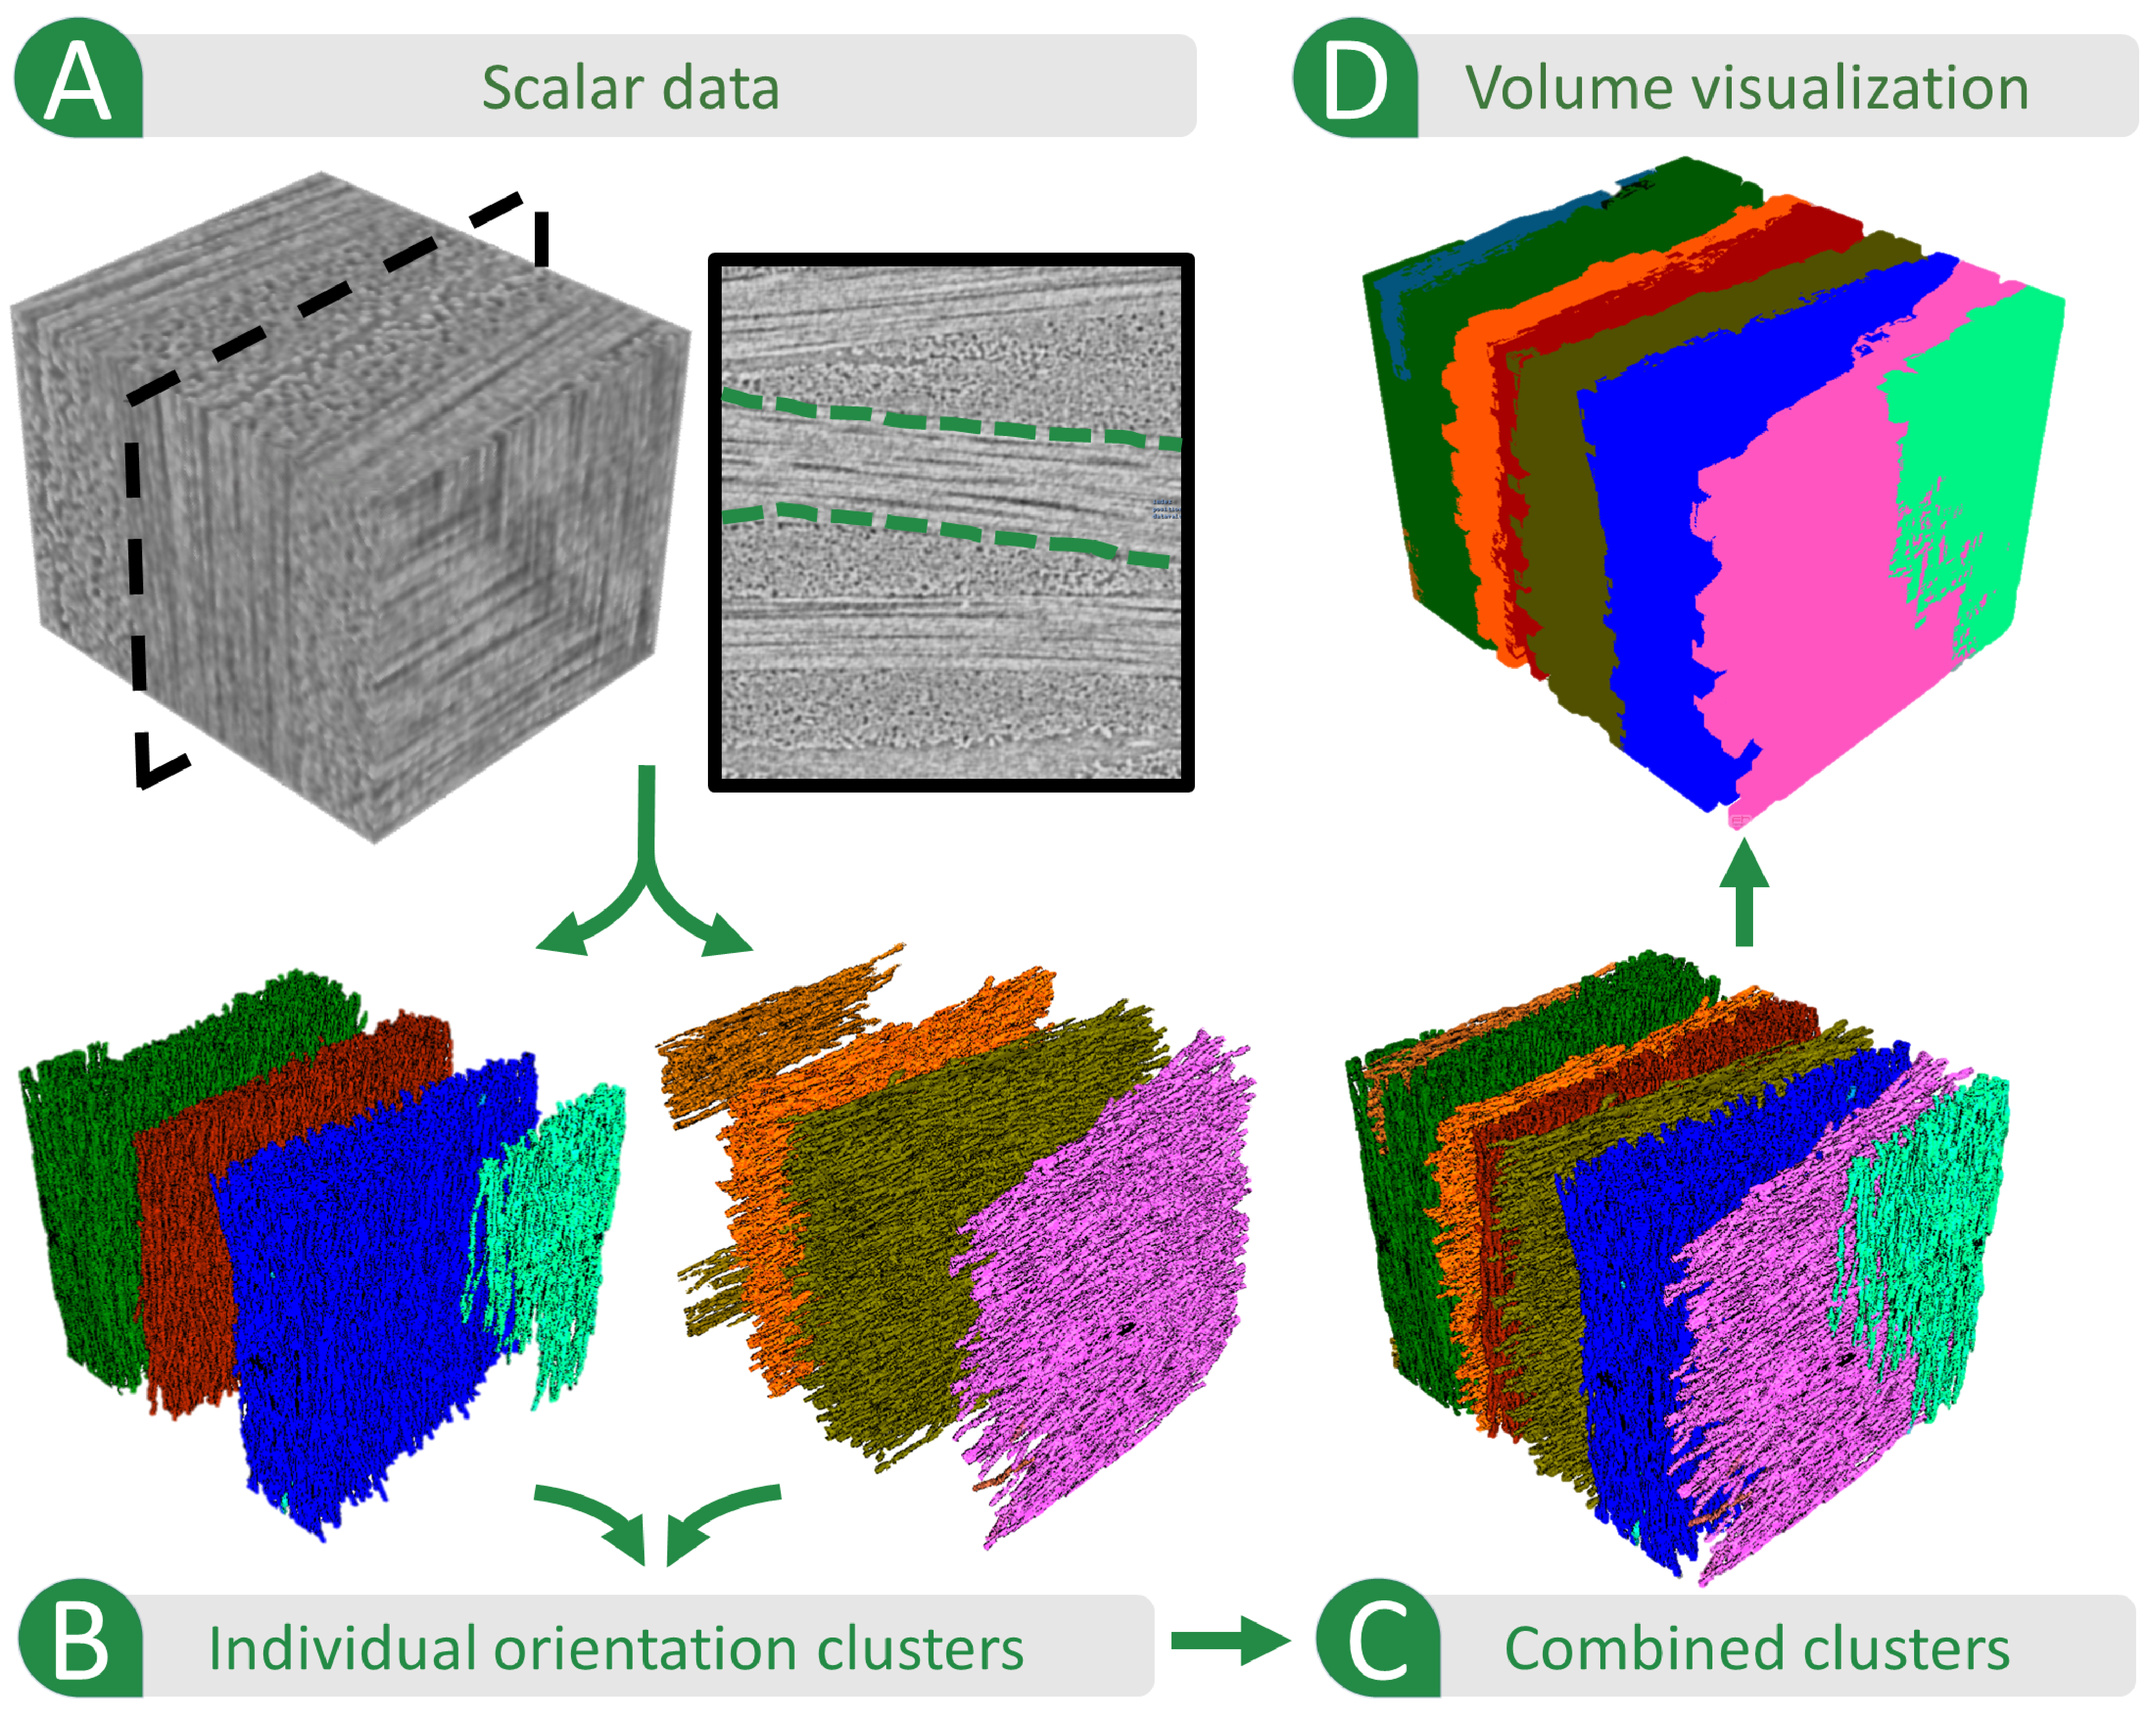
\includegraphics[width=\linewidth]{images/dataset2.eps}
	\caption{Data set with flat thin and compact bundles. (a) shows the volume rendering and a 2D slice with one of the boundaries marked in green, (b) shows the clusters according to individual orientation. (c) shows the complete result. (d) shows the voxelization of (c).}
	\label{fig:prepreg}
\end{figure} 